\documentclass[10pt]{beamer}

\input{/Users/daniel/Documents/LaTeX/beamer-style.tex}


\title{SGBD - 2\textsuperscript{e}}
\subtitle{Chapitre 3 - Langage de définition des données (LDD)}
\date{\today}
\author{Daniel Schreurs}
\institute{Haute École de Province de Liège}
%\titlegraphic{\hfill\includegraphics[height=1.5cm]{logo.eps}}


\setbeamertemplate{frame footer}{\insertsectionhead}

\begin{document}

\maketitle

\setbeamerfont{subsection in toc}{size=\small}
\setbeamerfont{subsubsection in toc}{size=\normalsize}
\setbeamertemplate{section in toc}[sections numbered]
\setbeamertemplate{subsection in toc}[subsections numbered]
\setbeamertemplate{subsubsection in toc}[subsubsections numbered]
\begin{frame}[allowframebreaks]{Table des matières du chapitre}
    \tableofcontents[subsectionstyle=show/show/hide,subsubsectionstyle=show/show/hide,]
\end{frame}

\section{Introduction}
\tocss
\subsection{Objectifs}
\begin{frame}{\secname : \subsecname}
    Dans ce chapitre, nous allons étudier les commandes principales pour :

    \begin{itemize}
        \item définir,
        \item modifier,
        \item supprimer
    \end{itemize}
    un objet d’une base de données relationnelle
\end{frame}

\subsection{BNF}
\begin{frame}{\secname : \subsecname}
    \begin{itemize}
        \item La forme de Backus-Naur (BNF : Backus-Naur Form) est une notation permettant de décrire les règles syntaxiques des langages de programmation.
        \item Elle est utilisée dans certains livres pour décrire le langage étudié, également par de nombreux logiciels d'analyse syntaxique.
        \item C'est une notation pour des grammaires formelles de type hors-contexte.
    \end{itemize}
\end{frame}

\begin{frame}{\secname : \subsecname}
    \begin{table}[]
        \begin{tabular}{|l|l|}
            \hline
            {Symbole}                   & {Signification}                                 \\ \hline
            {::=}                       & {Définit comme suit}                            \\ \hline
            {|}                         & {"ou" logique}                                  \\ \hline
            {\textless{}\textgreater{}} & {Concept (nom d'objet, valeur, …)}              \\ \hline
            {{[} {]}}                   & {Option possible, non obligatoire}              \\ \hline
            {\{ \}}                     & {Élément à choisir, liste d'éléments à choisir} \\ \hline
        \end{tabular}
    \end{table}
\end{frame}

\subsection{Avertissement}
\begin{frame}{\secname : \subsecname}
    \begin{alertblock}{Remarque très importante}
        Au cours théorique, nous voyons la norme SQL2.
        Au laboratoire, nous mettons en pratique dans l’environnement Oracle.
        Oracle n’implémente pas l’entièreté de la norme, en particulier, l’objet Domaine n’existe pas en Oracle !
    \end{alertblock}
\end{frame}



\section{Domaines}
\tocss
\subsection{Création}
\begin{frame}{\secname : \subsecname}
    \lstinputlisting[language=bnf,title=CREATE DOMAIN]{../exemples/CREATE-DOMAIN.bnf}
    \footnote{Attention, la valeur par défaut c'est $NULL$.}
\end{frame}

\subsection{Valeurs possibles}
\begin{frame}{\secname : \subsecname}
    Les valeurs possibles
    \begin{itemize}
        \item $Constante$ :   un nombre, une chaîne de caractères ou une date
        \item $USER$ :         nom de l'utilisateur (user name) du processus qui a lancé une session SQL interactive ou qui a lancé l'exécution d'un programme
        \item $NULL$ :         valeur indéfinie des bases de données
        \item $CURRENT\_DATE$ : la date du jour (année, mois, jour)
        \item $CURRENT\_TIME$ : le temps courant (heure, minute, seconde)
        \item $CURRENT\_TiMESTAMP$ : la date et le temps courants (jour, mois, année, heure, minute, seconde)
    \end{itemize}
\end{frame}

\subsection{CHAR et VARCHAR}
\begin{frame}{\secname : \subsecname}
    Différence entre CHAR et VARCHAR :
    \begin{itemize}
        \item CHAR(40) : la taille du champ aura toujours la longueur 40, la longueur est fixe
        \item VARCHAR(40) : le 40 représente la taille maximale permise pour le champ, si on ne met que 1 caractère, on n'utilisera que la place nécessaire pour 1 caractère.
    \end{itemize}
\end{frame}

\begin{frame}{\secname : \subsecname}
    Types :
    \begin{itemize}
        \item SMALLINT : 2 bytes
        \item INTEGER : 4 byes
        \item NUMERIC/DECIMAL : la différence est la représentation de la donnée en mémoire
        \item DECIMAL : (nombre de chiffres dans le nombre + 1) / 2 $\implies$ nb bytes nécessaires
        \item NUMERIC : 1 byte par chiffre
    \end{itemize}
\end{frame}

\subsection{Type DATE}
\begin{frame}{\secname : \subsecname}
    SQL2 a apporté une extension au type DATE.
    \begin{itemize}
        \item Le type datetime
              \begin{itemize}
                  \item DATE (ex. 1957-01-11)
                  \item TIME (ex. 21:30:15.54)
                  \item TIMESTAMP (ex. 1957-01-11:21:30:15.54)
              \end{itemize}
        \item Le type interval\footnote{peut être négatif}.
              \begin{itemize}
                  \item Année-mois
                  \item Jour-temps
              \end{itemize}
    \end{itemize}
\end{frame}

\begin{frame}{\secname : \subsecname}
    \begin{itemize}
        \item Les intervalles Année-Mois comprennent :
              \begin{itemize}
                  \item YEAR
                  \item YEAR TO MONTH
                  \item MONTH
              \end{itemize}
        \item Les intervalles Jour-Temps  comprennent :
              \begin{itemize}
                  \item DAY
                  \item DAY TO HOUR
                  \item DAY TO MINUTE
                  \item DAY TO SECOND
                  \item HOUR
                  \item HOUR TO MINUTE
                  \item HOUR TO SECOND
                  \item MINUTE
                  \item MINUTE TO SECOND
                  \item SECOND
              \end{itemize}
    \end{itemize}
\end{frame}

\begin{frame}{\secname : \subsecname}
    \lstinputlisting[language=plsql,title=Exemple : CREATE DOMAIN]{../exemples/CREATE-DOMAIN.sql}
\end{frame}

\section{Relations}
\tocss
\subsection{CREATE TABLE}
\begin{frame}{\secname : \subsecname}
    \lstinputlisting[language=plsql,title=CREATE TABLE]{../exemples/CREATE-table.bnf}
\end{frame}

\begin{frame}{\secname : \subsecname}
    \begin{itemize}
        \item Dans un même schéma, le nom des tables doit être unique
        \item Avec oracle : un type par colonnes\footnote{Puisque la notion de domaine n'existe pas en Oracle}.
        \item On peut avoir plusieurs contraintes sur une même colonne
        \item On peut préciser des contraintes au niveau de la colonne en cours
        \item $CHECK$ permet de mettre des contraintes applicatives.\footnote{On peut mettre une condition composée avec des ET et des OU.}
        \item Pour les clés étrangères :  ON DELETE et ON UPDATE.
    \end{itemize}
\end{frame}

\subsection{CREATE CONSTRAINT}
\begin{frame}{\secname : \subsecname}
    \lstinputlisting[language=plsql,title=CREATE CONSTRAINT]{../exemples/CREATE-CONSTRAINT.bnf}\footnote{Le mode de la contrainte est différé ou non.  Par défaut, une contrainte n'est pas différée.  Elle est vérifiée au moment de l'exécution de l'instruction d'insertion ou mise à jour.  Si la contrainte est différée, elle est contrôlée au moment du commit.
    }
\end{frame}

\begin{frame}{\secname : \subsecname}
    \begin{itemize}
        \item Par défaut, une colonne est "nullable" (NULL)
        \item L'ensemble formé par les noms des colonnes doit être unique au sein de la table
        \item L'ensemble formé par le nom des contraintes doit être unique au sein du schéma
    \end{itemize}
\end{frame}

\begin{frame}{\secname : \subsecname}
    \begin{itemize}
        \item La casse, n'a pas d'importance au niveau des mots-clés de SQL, des noms de tables, colonnes, index, etc.
        \item La casse a une incidence majeure dans les expressions de comparaison entre colonnes et valeurs
    \end{itemize}
\end{frame}
\subsection{Formes de contraintes}
\begin{frame}{\secname : \subsecname}
    Deux formes de contraintes :
    \begin{itemize}
        \item Une contrainte de colonne permet d’associer une contrainte à UNE colonne
        \item Une contrainte de table permet de définir une contrainte au niveau de la table, et donc faire intervenir plusieurs colonnes :
              \begin{itemize}
                  \item Clé primaire ou étrangère composée de plusieurs colonnes
                  \item Comparaison des valeurs contenues dans 2 colonnes (date de naissance $\leq$ date décès)
              \end{itemize}
    \end{itemize}
\end{frame}

\subsection{Types de contraintes}
\begin{frame}{\secname : \subsecname}
    Plusieurs types de contraintes :
    \begin{itemize}
        \item Sur les valeurs directement : DEFAULT / NOT NULL / UNIQUE
        \item Sur les intégrités : PRIMARY KEY, FOREIGN KEY, SK (secondary key)
        \item Sur des conditions à remplir : CHECK
    \end{itemize}
\end{frame}

\subsection{Bonnes pratiques}
\begin{frame}{\secname : \subsecname}
    Sans la clause CONSTRAINT, SQL génère automatiquement un nom pour chaque contrainte.
    Il est donc vivement conseillé d’utiliser systématiquement la clause CONSTRAINT
    \lstinputlisting[language=plsql,title=Exemple : nom de contrainte]{../exemples/exemple-constraint.sql}
\end{frame}

\subsection{Contraintes sur les valeurs propres}
\begin{frame}{\secname : \subsecname}
    \begin{itemize}
        \item Principe : restreindre les conditions d'acceptation des données dans la ou les colonnes
        \item 3 contraintes de valeurs propres : NOT NULL, DEFAULT, CHECK
    \end{itemize}
    \lstinputlisting[language=bnf,title=Exemple : nom de contrainte]{../exemples/constraint.bnf}
\end{frame}

\begin{frame}{\secname : \subsecname}
    \begin{itemize}
        \item Il ne faut pas confondre NULL qui est une ABSENCE de valeur ou un ensemble vide avec :
              \begin{itemize}
                  \item Un numérique dont la valeur est zéro (qui est une valeur)
                  \item Une chaîne de caractères vide (qui a un sens)
              \end{itemize}
    \end{itemize}
    NULL est un marqueur
\end{frame}

\begin{frame}{\secname : \subsecname}
    Valeurs par défaut d'une colonne (expression\_defaut)

    \begin{itemize}
        \item Constantes les plus courantes : $ CURRENT\_DATE,CURRENT\_TIME,CURRENT\_TIMESTAMP $ etc.
        \item Toute valeur scalaire définie par l'utilisateur
        \item Remarque : si une colonne a une valeur par défaut et est définie par un domaine ayant une valeur par défaut, la première prend le pas sur la seconde.
    \end{itemize}
\end{frame}

\begin{frame}{\secname : \subsecname}
    Contrainte de validation (CHECK)
    \begin{itemize}
        \item Permet de restreindre les valeurs acceptables pour la colonne en appliquant un PREDICAT.
        \item Si le prédicat est VRAI, l'instruction est acceptée et la valeur de la colonne du tuple est validée
        \item Ce type de contrainte peut viser à valider plusieurs colonnes simultanément (contrainte de table) ou une seule colonne (contrainte de colonne)
    \end{itemize}
\end{frame}

\begin{frame}{\secname : \subsecname}
    Contrainte de validation (CHECK) peut contenir :
    \begin{itemize}
        \item Des valeurs explicites
        \item Le marqueur NULL
        \item Des valeurs sous forme de fonction SQL ou UDF
        \item Des opérateurs algébriques $+, -, *, /$
        \item Des concaténations de chaînes $||$
        \item Des opérateurs de comparaisons $>, <, <=, >=, <>$
        \item Des connecteurs logiques $AND, OR$
        \item L'opérateur de négation $NOT$
        \item La hiérarchisation des opérateurs à l'aide de parenthèses
        \item Des expressions SQL spécifiques, y compris d'appel à d'autres tables
    \end{itemize}
\end{frame}

\begin{frame}{\secname : \subsecname}
    Opérateurs SQL
    \begin{table}[]
        \begin{tabular}{|l|l|}
            \hline
            {Opérateur} & {Signification}                                           \\ \hline
            {BETWEEN}   & {Plage de valeurs (bornes comprises dans l'intervalle)}   \\ \hline
            {LIKE}      & {Comparaison partielle de chaines de caractères (\%, \_)} \\ \hline
            {IN}        & {Liste de valeurs possibles}                              \\ \hline
            {CASE}      & {Branchement de différentes valeurs}                      \\ \hline
            {OVERLAPS}  & {Recouvrement de périodes}                                \\ \hline
            {SIMILAR}   & {Expression rationnelle}                                  \\ \hline
        \end{tabular}
    \end{table}
\end{frame}
\subsection{Contraintes d'intégrités}
\begin{frame}{\secname : \subsecname}
    Contraintes portant sur les intégrités\footnote{Ces contraintes ne peuvent être bâties sur une colonne de type LOB (CLOB/BLOB/NCLOB) ou de type objet.}
    \begin{itemize}
        \item Permettent de restreindre les valeurs des données de différentes colonnes par rapport à un ensemble de données pris dans l'intégralité des lignes d'une table.
        \item 3 types de contraintes de clé :
              \begin{itemize}
                  \item Primary key
                  \item Foreign key
                  \item Unique
              \end{itemize}
    \end{itemize}
\end{frame}
\begin{frame}{\secname : \subsecname}
    \lstinputlisting[language=bnf,title=Contrainte de colonne]{../exemples/constraint--col.bnf}
    \lstinputlisting[language=bnf,title=Contrainte de table]{../exemples/constraint--table.bnf}
\end{frame}

\subsection{Clé primaire}
\begin{frame}{\secname : \subsecname}
    \begin{alertblock}{Important}
        Il ne peut y avoir qu'une seule contrainte de clé primaire par table
    \end{alertblock}
    \begin{itemize}
        \item Les colonnes participant à la clé primaire ne peuvent pas être marquée "NULLable"
        \item Les colonnes faisant partie de la définition d'une contrainte de clé primaire seront automatiquement basculées à NOT NULL
    \end{itemize}
\end{frame}

\subsection{Clé subrogée (UNIQUE)}
\begin{frame}{\secname : \subsecname}
    \begin{itemize}
        \item Impose que les occurrences de toutes les valeurs renseignées pour la ou les colonnes faisant partie de cette clé soient différentes (sans doublons)
        \item Marqueur NULL peut être présent plusieurs fois;
        \item Autant de contraintes UNIQUE que l'on veut
        \item La contrainte UNIQUE n'impose pas le NOT NULL
    \end{itemize}
\end{frame}

\subsection{Clé étrangère}
\begin{frame}{\secname : \subsecname}
    \begin{itemize}
        \item Permet de lier les tables du modèle relationnel
        \item Permet de vérifier la présence des valeurs dans les colonnes d'une autre contrainte (primaire OU subrogée) prise dans une autre table\footnote{Dite table mère}
        \item Lié à une clé primaire ou subrogée
    \end{itemize}
\end{frame}




\begin{frame}{\secname : \subsecname}
    \lstinputlisting[language=bnf,title=Contrainte FK]{../exemples/constraint--fk.bnf}
\end{frame}

\begin{frame}{\secname : \subsecname}
    \begin{itemize}
        \item Pour insérer ou modifier une valeur de colonne pourvue d'une clé étrangère, la valeur (référençante) doit exister dans la table mère (valeur référencée)
        \item Types des colonnes : domaines compatibles
        \item Les noms des colonnes référençantes et référencées peuvent être différents.\footnote{Mais il est conseillé de leur donner le même nom car elles sont sémantiquement liées.  Cela permet également les jointures naturelles.}
    \end{itemize}
\end{frame}

\begin{frame}{\secname : \subsecname}
    \lstinputlisting[language=plsql,title=Exemple contrainte 1]{../exemples/constraint--short.sql}
    Deux manières équivalentes
    \lstinputlisting[language=plsql,title=Exemple contrainte 2]{../exemples/constraint--full.sql}
\end{frame}

\subsection{Tables temporaires}
\begin{frame}{\secname : \subsecname}
    Il est également possible de créer des tables temporaires :
    \lstinputlisting[language=bnf,title=Exemple contrainte 2]{../exemples/CREATE-TEMPORARY-TABLE.bnf}
    Ces tables :
    \begin{itemize}
        \item Sont vides au début de chaque session SQL,
        \item Peuvent être vidées à chaque COMMIT,
        \item Sont supprimées automatiquement à la fin de la session SQL
        \item Sont instanciées lors de la première référence (chaque session possède sa propre version, donc pas d’accès concurrents !)
    \end{itemize}
\end{frame}

\subsection{Exercice}
\begin{frame}{\secname : \subsecname}
    \begin{figure}
        \begin{center}
            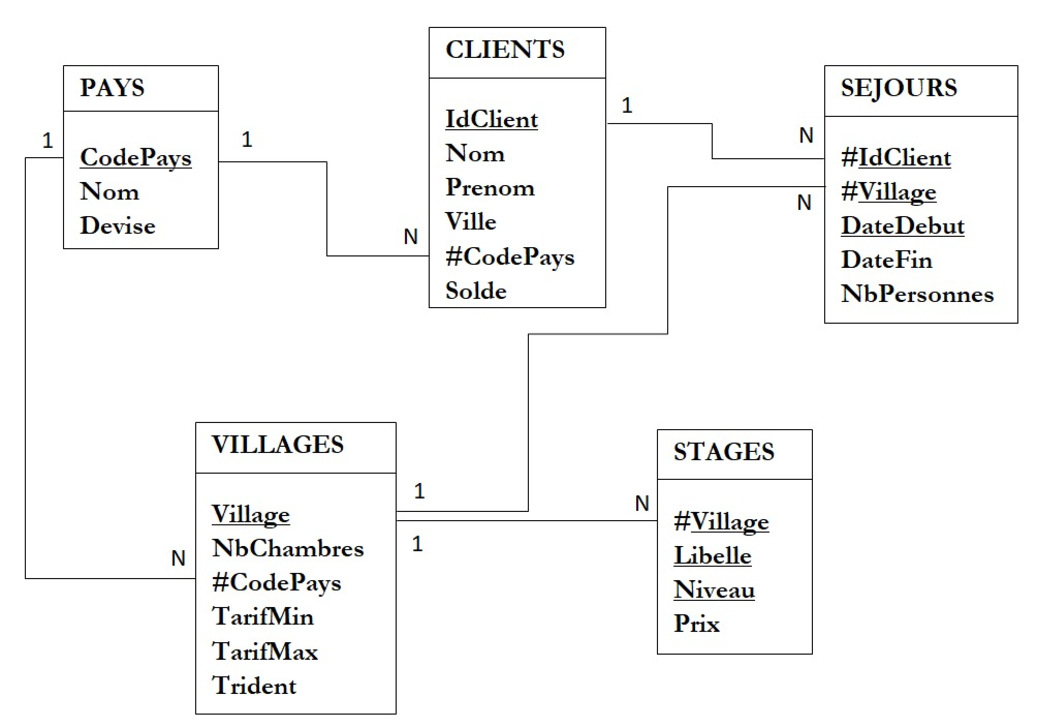
\includegraphics[width=0.8\textwidth]{../assets/img/pays-exercice.pdf}
            \label{Fig:pays-exercice}
        \end{center}
    \end{figure}
\end{frame}
\begin{frame}{\secname : \subsecname}
    \begin{figure}
        \begin{center}
            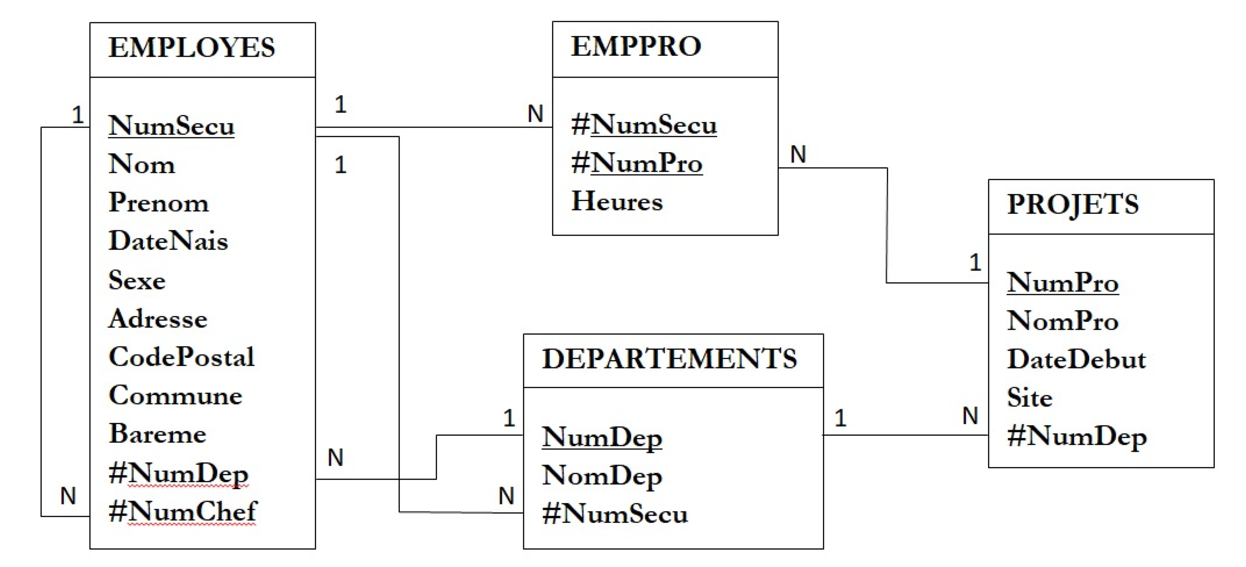
\includegraphics[width=0.8\textwidth]{../assets/img/employes-exercice.pdf}
            \label{Fig:employes-exercice}
        \end{center}
    \end{figure}
\end{frame}

\section{Bases de données}
\tocss
\subsection{Généralités}
\begin{frame}{\secname : \subsecname}
    \begin{itemize}
        \item La norme SQL2 ne définit pas formellement la notion de \emph{base de données};
        \item Elle indique que toutes les opérations SQL doivent être exécutées au sein d'un environnement appelé SQL-environment;
        \item Un environnement peut contenir plusieurs catalogues. Chaque catalogue est constitué d'un ensemble de schémas;
        \item Un schéma est une collection de domaines, de relations, de contraintes, de vues et de privilèges\footnote{Notion la plus proche d'une base de données};
        \item La norme ne définit pas de mécanismes explicites de création et de destruction des catalogues.
    \end{itemize}
\end{frame}

\begin{frame}{\secname : \subsecname}
    \lstinputlisting[language=bnf,title=CREATE SCHEMA]{../exemples/CREATE-SCHEMA.bnf}
    $ListeElementsSchema$ permet de définir les domaines, les relations, les vues, les contraintes et les autorisations d'accès contenus dans le schéma.
    Il est possible d'effectuer des opérations entre objets de schémas différents :
    $Test.Bibliotheque.Membres$ désigne la table Membres du schéma Bibliothèque du catalogue Test
\end{frame}

\subsection{Généralités - Oracle}
\begin{frame}{\secname : \subsecname}
    \begin{itemize}
        \item Une base de données Oracle est constituée d'une collection de schémas (users).
        \item Un schéma contient des objets du monde relationnel: table, vue, index, ainsi que des déclencheurs, fonctions, procédures stockées et packages...
        \item Ces schémas sont répartis dans des zones logiques appelées tablespaces constituées de segments (segments) composés de différentes extension (extents) organisées en blocs (blocks).
    \end{itemize}
\end{frame}

\begin{frame}{\secname : \subsecname}
    Aperçu des instructions Oracle pour créer une base de données, un tablespace,...
    \lstinputlisting[language=plsql,title=Quelques instructions Oracle]{../exemples/cmd-oracle.sql}
\end{frame}

\subsection{Information schema}
\begin{frame}{\secname : \subsecname}
    \begin{itemize}
        \item Chaque catalogue contient un schéma spécial, \emph{Information schema} qui contient la définition de tous les objets inclus dans les différentes schémas du catalogue.
        \item Ce schéma est appelé \emph{dictionnaire} ou \emph{méta-base}
        \item Il comporte un ensemble de tables, vues et contraintes créées et maintenues automatiquement par le SGBD.
        \item Il est accessible (pour consultation uniquement) aux utilisateurs de la base au moyen de SQL.
    \end{itemize}
\end{frame}

\begin{frame}{\secname : \subsecname}
    Principales tables et vues contenues dans le dictionnaire :
    \begin{itemize}
        \item Informations générales sur la base
        \item Domaines et colonnes
        \item Tables et vues
        \item Droit d'accès
        \item Contraintes
    \end{itemize}
\end{frame}

\begin{frame}{\secname : \subsecname}
    \begin{table}[]
        \resizebox{\textwidth}{!}{%
            \begin{tabular}{|l|l|}
                \hline
                Nom de la table                    & Informations                                                   \\ \hline
                INFORMATION\_SCHEMA\_CATALOG\_NAME & \begin{tabular}[c]{@{}l@{}}Table d'une ligne et une colonne qui contient le nom \\ du catalogue dans lequel le information schema réside.\end{tabular}                                     \\ \hline
                SCHEMATA                           & Contient la liste des schémas créés par l'utilisateur courant. \\ \hline
            \end{tabular}}
        \caption*{Informations générales sur la base}
    \end{table}
\end{frame}

\begin{frame}{\secname : \subsecname}
    \begin{table}[]
        \resizebox{\textwidth}{!}{%
            \begin{tabular}{|l|l|}
                \hline
                DOMAINS               & Contient la liste des domaines                        \\ \hline
                COLUMNS               & Contient la liste des colonnes des tables et des vues \\ \hline
                COLUMN\_DOMAIN\_USAGE & Contient le domaine de définition de chaque colonne   \\ \hline
            \end{tabular}}
        \caption*{Domaines et colonnes}
    \end{table}
\end{frame}

\begin{frame}{\secname : \subsecname}
    \begin{table}[]
        \resizebox{\textwidth}{!}{%
            \begin{tabular}{|l|l|}
                \hline
                TABLES              & contient le liste des tables et vues                                 \\ \hline
                VIEWS               & contient la définition des vues                                      \\ \hline
                VIEW\_TABLE\_USAGE  & indique les tables (ou les vues) dont dépend chaque vue              \\ \hline
                VIEW\_COLUMN\_USAGE & indique les colonnes des tables (ou des vues) dont dépend chaque vue
                \\ \hline
            \end{tabular}}
        \caption*{Tables et vues}
    \end{table}
\end{frame}

\begin{frame}{\secname : \subsecname}
    \begin{table}[]
        \resizebox{\textwidth}{!}{%
            \begin{tabular}{|l|l|}
                \hline
                TABLE\_PRIVILEGES  & liste des privilèges d'accès aux tables ou aux vues \\ \hline
                COLUMN\_PRIVILEGES & liste des privilèges d'accès aux colonnes           \\ \hline
                USAGE\_PRIVILEGES  & liste des privilèges d'accès aux domaines           \\ \hline
            \end{tabular}}
        \caption*{Droit d'accès}
    \end{table}
\end{frame}

\begin{frame}{\secname : \subsecname}
    \begin{table}[]
        \resizebox{\textwidth}{!}{%
            \begin{tabular}{|l|l|}
                \hline
                DOMAIN\_CONSTRAINTS      & liste des contraintes portant sur les domaines                            \\ \hline
                TABLE\_CONSTRAINTS       & liste des contraintes portant sur les tables                              \\ \hline
                REFERENTIAL\_CONSTRAINTS & liste des contraintes référentielles                                      \\ \hline
                CHECK\_CONSTRAINTS       & liste des contraintes de type CHECK                                       \\ \hline
                KEY\_COLUMN\_USAGE       & liste des colonnes participant à une clé candidate ou à une clé étrangère \\ \hline
                ASSERTIONS               & liste des contraintes générales                                           \\ \hline
                CONSTRAINT\_TABLE\_USAGE & liste des tables intervenant dans une contrainte                          \\ \hline
                CONSTRAINT\_TABLE\_USAGE & liste des colonnes intervenant dans une contrainte                        \\ \hline
            \end{tabular}}
        \caption*{Contraintes}
    \end{table}
\end{frame}
\subsection{Information schema - Oracle}
\begin{frame}{\secname : \subsecname}
    \begin{figure}
        \begin{center}
            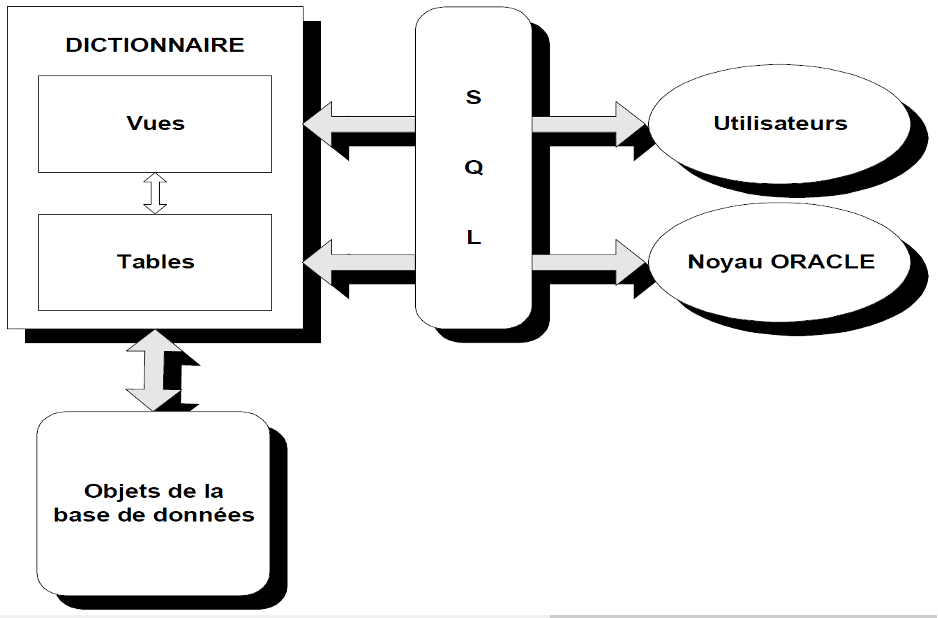
\includegraphics[width=0.5\textwidth]{../assets/img/dictionnaire--oracle.png}
            \caption*{Structure et utilisation du dictionnaire de données en Oracle}
            \label{Fig:dictionnaire--oracle}
        \end{center}
    \end{figure}
\end{frame}

\begin{frame}{\secname : \subsecname}
    \begin{itemize}
        \item Les vues relatives aux objets d'un utilisateur :
              \begin{itemize}
                  \item $USER\_TABLES$
                  \item $USER\_OBJECTS$
                  \item ...
              \end{itemize}
        \item Les vues relatives aux objets accessibles à un utilisateur :
              \begin{itemize}
                  \item $ALL\_TABLES$
                  \item $ALL\_OBJECTS$
                  \item ...
              \end{itemize}
        \item Les vues relatives aux administrateurs :
              \begin{itemize}
                  \item $DBA\_DATA\_FILES$
                  \item $DBA\_CATALOG$
              \end{itemize}

        \item Les vues relatives au suivi des performances :
              \begin{itemize}
                  \item $V\$LOGFILE$
                  \item $V\$SESSION$
              \end{itemize}
    \end{itemize}
\end{frame}
\section{Index}
\tocss
\subsection{La méthode séquentielle}
\begin{frame}{\secname : \subsecname}
    La méthode séquentielle est très simple et ne nécessite aucune gestion supplémentaire pour le SGBD.
    Elle convient bien pour :
    \begin{itemize}
        \item Les parcours complets
        \item Les opérations d'ajouts massifs
        \item Elle devient vite inefficace pour résoudre des requêtes contenant des jointures ou n'extrayant que peu de tuples d'une table.
    \end{itemize}
\end{frame}

\begin{frame}{\secname : \subsecname}
    \metroset{block=fill}
    \begin{alertblock}{Important}
        Augmenter la rapidité d'accès aux tuples en proposant un accès plus direct que l'accès séquentiel.\footnote{Dès qu'on définit la clé primaire, EN ORACLE (pas dans la norme), un index est créé sur cette clé primaire.}
    \end{alertblock}
    \begin{itemize}
        \item Un index peut être défini sur plusieurs colonnes ? \textbf{V}/F
        \item Un index ne porte que sur une seule relation ? V/\textbf{F}
        \item Une relation peut posséder plusieurs index ? \textbf{V}/F\footnote{Attention, lors des mises à jour, les index doivent aussi être mis à jour $\implies$ plus lent.}
    \end{itemize}
\end{frame}

\subsection{Index hiérarchiques}
\begin{frame}{\secname : \subsecname}
    Un index peut être défini sur une seule relation, à partir d'une ou plusieurs colonnes.
    \lstinputlisting[language=bnf,title=CREATE INDEX ]{../exemples/CREATE-INDEX.bnf}
    \begin{itemize}
        \item Il est possible de définir plusieurs index sur une même relation, mais ce n'est pas toujours souhaitable.
        \item Un index hiérarchique ressemble à un arbre dont les feuilles pousseraient vers le bas et peut être comparé à un fichier séquentiel indexé.
        \item Pratiquement tous les SGBD (dont Oracle) utilisent les index hérarchiques B-TREE.
    \end{itemize}
\end{frame}

\begin{frame}{\secname : \subsecname}
    \begin{figure}
        \begin{center}
            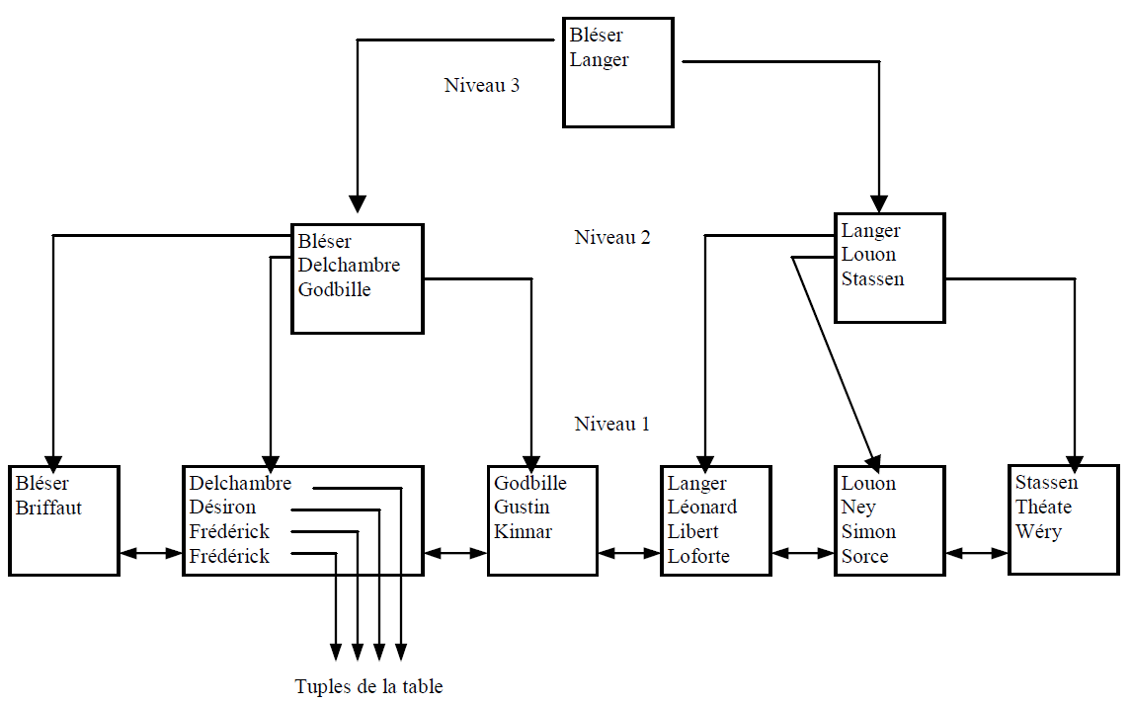
\includegraphics[width=0.8\textwidth]{../assets/img/index-B-TREE.png}
            \caption*{Index hiérarchiques}
            \label{Fig:index-B-TREE}
        \end{center}
    \end{figure}
\end{frame}

\begin{frame}{\secname : \subsecname}
    \metroset{block=fill}
    \begin{alertblock}{Résumé des principales caractéristiques}
        \begin{itemize}
            \item Offrent des recherches rapides en fonction d'une valeur précise de la clé ou d'une plage de valeurs pour la clé
            \item conviennent pour les colonnes qui ont un grand nombre de valeurs différentes et qui interviennent dans les critères de recherches ou de jointures
            \item en pratique, on en définit toujours pour les clés primaires et les clés étrangères
        \end{itemize}
    \end{alertblock}
\end{frame}



\subsection{Cluster indexé}
\begin{frame}{\secname : \subsecname}
    Un cluster contient les tuples d'une ou plusieurs tables qui possèdent au moins une colonne commune.
    Les tuples qui partagent la même valeur pour ces colonnes communes sont physiquement stockés ensemble dans la base de données.

    \metroset{block=fill}
    \begin{alertblock}{Important}
        Ce type de structure optimise le temps nécessaire aux opérations de jointure.
    \end{alertblock}
    \lstinputlisting[language=plsql,title=Cluster indexé]{../exemples/CREATE-INDEX--cluster.sql}
\end{frame}

\begin{frame}{\secname : \subsecname}
    \lstinputlisting[language=plsql,title=Cluster indexé]{../exemples/CREATE-INDEX--cluster-2.sql}
\end{frame}

\begin{frame}{\secname : \subsecname}
    \metroset{block=fill}
    \begin{alertblock}{Résumé des principales caractéristiques}
        \begin{itemize}
            \item En regroupant physiquement les lignes de plusieurs tables, améliorent les temps de jointures.
            \item MAIS pénalisent les parcours séquentiels
        \end{itemize}
    \end{alertblock}
\end{frame}

\subsection{Index haché}
\begin{frame}{\secname : \subsecname}
    \begin{itemize}
        \item Le SGBD applique une fonction mathématique, appelée fonction de hachage, sur une clé.  Le résultat est un numéro de bloc dans un fichier ou zone de stockage. Le tuple
        \item Le numéro de bloc dépend du nombre de blocs initialement alloués à la zone de stockage et, évidemment, de la clé.
        \item Il ne peut donc y avoir qu'un seul hachage par relation.
        \item En théorie, cette technique permet d'accéder à un tuple en une entré/sortie.
    \end{itemize}
\end{frame}

\begin{frame}{\secname : \subsecname}
    \metroset{block=fill}
    \begin{alertblock}{Important}
        Problème de collisions\footnote{Les collisions augmentent le nombre d'entrées/sorties nécessaires à la recherche d'un tuple et brisent l'ordre logique.} :
        \begin{itemize}
            \item Chaînage des collisions
            \item Application d'une fonction secondaire
        \end{itemize}
    \end{alertblock}
\end{frame}
\begin{frame}{\secname : \subsecname}
    \begin{itemize}
        \item Pour limiter les collisions au maximum, le concepteur de la base de données doit choisir un nombre de blocs initiaux suffisamment grand.  Pour une grande relation, il n'est pas rare de définir une réserve d'espace de 50%.
        \item La répartition des tuples dans les blocs sera d'autant meilleure que le nombre de clés différentes est plus élevé.
        \item Le hachage à partir d'une colonne contenant beaucoup de valeurs NULL est donc à proscrire.
    \end{itemize}
\end{frame}

\begin{frame}{\secname : \subsecname}
    \begin{itemize}
        \item Exemple : le hachage est réalisé à partir de la colonne $Num\_Article$. Il y aura 25000 valeurs hachées. On aura donc des collisions dès que la table Articles contiendra plus de 25000 tuples.
    \end{itemize}
    \lstinputlisting[language=plsql,title=Cluster indexé]{../exemples/CREATE-INDEX--hash.sql}
\end{frame}

\begin{frame}{\secname : \subsecname}
    \metroset{block=fill}
    \begin{alertblock}{Résumé}
        Permettent en une seule opération d'entrée/sortie, de retrouver un tuple dont on donne la valeur de la clé.
    \end{alertblock}
\end{frame}

\subsection{Index à matrices binaires}
\begin{frame}{\secname : \subsecname}
    \begin{itemize}
        \item Colonnes qui ne possèdent que quelques valeurs distinctes
        \item Un index à matrices binaires est constitué d'un ensemble de matrices dont les éléments prennent uniquement les valeurs 1 ou 0
        \item Une matrice est toujours associée à une des colonnes de la table indexée
        \item À chaque ligne de chaque matrice correspond une et une seule ligne de la table
        \item Le nombre de colonnes de la matrice associée à la colonne C est égal au nombre de valeurs différentes présentes dans la colonne C
    \end{itemize}
\end{frame}

\begin{frame}{\secname : \subsecname}
    \begin{figure}
        \begin{center}
            \includegraphics[width=0.70\textwidth]{../assets/img/Index à matrices binaires.png}
            \caption*{Index à matrices binaires}
            \label{Fig:Index à matrices binaires}
        \end{center}
    \end{figure}
\end{frame}

\begin{frame}{\secname : \subsecname}
    \metroset{block=fill}
    \begin{alertblock}{Important}
        Ce type d'index est souvent utilisé dans le contexte des data warehouse dans lequel on manipule couramment des tables de plusieurs millions de lignes mais dont les colonnes ne contiennent que quelques valeurs différentes.
    \end{alertblock}
\end{frame}


\begin{frame}{\secname : \subsecname}
    \lstinputlisting[language=plsql, title=Création d'un index bitmap en Oracle]{../exemples/CREATE-INDEX--bitmap.sql}
\end{frame}

\begin{frame}{\secname : \subsecname}
    \metroset{block=fill}
    \begin{alertblock}{Résumé des principales caractéristiques}
        \begin{itemize}
            \item sont utiles pour les requêtes de comptage en fonction de critères portant sur plusieurs colonnes contenant peu de valeurs différentes
            \item sont utilisés pour de grandes tables
        \end{itemize}
    \end{alertblock}
\end{frame}

\subsection{Index basé sur une fonction}
\begin{frame}{\secname : \subsecname}
    À partir d'une fonction ou d'une expression faisant intervenir des colonnes de la table indexée.\footnote{La fonction peut être une fonction SQL, PL/SQL ou externe.}
    \lstinputlisting[language=plsql, title=Création d'un index bitmap en Oracle]{../exemples/CREATE-INDEX--bitmap-2.sql}
\end{frame}

\section{Suppression d’un objet}
\tocss
\subsection{DROP DOMAIN}
\begin{frame}{\secname : \subsecname}
    \lstinputlisting[language=bnf, title=DROP DOMAIN]{../exemples/DROP-SCHEMA.bnf}
    \begin{itemize}
        \item RESTRICT : interdit la suppression
              \begin{itemize}
                  \item S'il y a des objets contenus
                  \item S'il est référencé par un autre schéma ou routine
              \end{itemize}
        \item CASCADE : supprime
              \begin{itemize}
                  \item Tous les objets contenus
                  \item Tous les objets externes au schéma mais y faisant référence
              \end{itemize}
    \end{itemize}
\end{frame}

\begin{frame}{\secname : \subsecname}
    \begin{itemize}
        \item Il est impossible de supprimer un domaine qui est encore utilisé dans la définition d'une table
        \item Il est impossible de supprimer un index qui est utilisé en même temps dans une autre requête
        \item DROP DATABASE efface physiquement tout ce qui concerne la base de donnée
    \end{itemize}
\end{frame}

\begin{frame}{\secname : \subsecname}
    \begin{itemize}
        \item DROP TABLE efface la table : ses données ET sa définition
        \item Si on utilise l'option RESTRICT, il est impossible de supprimer la table si :
              \begin{itemize}
                  \item La table est utilisée en même temps dans une autre requête (une sélection par ex.)
                  \item La table est utilisée dans la construction d'une vue
                  \item La table est référencée par une autre table (contrainte de référence)
              \end{itemize}
        \item Si on utilise la clause CASCADE, l'effacement de la table entraîne automatiquement la suppression de tous les objets qui lui faisaient référence (index, vue, contrainte, déclencheur)
    \end{itemize}
\end{frame}

\section{Modification de la définition d’un objet}
\tocss
\subsection{Modification de la définition d'un domaine}
\begin{frame}{\secname : \subsecname}
    \begin{itemize}
        \item Syntaxe identique à celle de CREATE DOMAIN dans laquelle on remplace CREATE par ALTER
        \item Intérêt : d'un seul coup, on modifie la définition de toutes les relations faisant référence au domaine modifié !
    \end{itemize}
\end{frame}
\subsection{Modification de la définition d'un table}
\begin{frame}{\secname : \subsecname}
    \begin{itemize}
        \item Permet d'ajouter de nouvelles colonnes, d'ajouter des contraintes (au niveau colonne ou table), de modifier des colonnes, de supprimer des colonnes et de supprimer des contraintes
        \item Ne permet pas de modifier une contrainte : il faut d'abord la supprimer puis la recréer.
    \end{itemize}
\end{frame}

\begin{frame}{\secname : \subsecname}
    \lstinputlisting[language=bnf, title=Modification de la définition d'un table]{../exemples/ALTER-TABLE.bnf}
\end{frame}

\begin{frame}{\secname : \subsecname}
    On ne peut pas modifier ou supprimer une colonne lorsqu'une des conditions suivantes est remplie :
    \begin{itemize}
        \item Elle est utilisée dans une vue
        \item Un index est basé sur la colonne
        \item La base de données contient une contrainte qui fait référence à la colonne
        \item ALTER TABLE échoue si on ajoute une contrainte qui n'est pas satisfaite
    \end{itemize}
\end{frame}





\end{document}
